% Section content template for individual Educative lessons
% This file contains the actual content for a specific section
% Generated from Educative API section content

% Section: Use Case Diagram for the Parking Lot
% Section ID: 5098525681778688
% Section Slug: use-case-diagram-for-the-parking-lot
% Generated: 2025-12-11T13:39:26.499028

Let's build the parking lot system's use case diagram and understand the relationships between its main actors and functions. First , we'll define the different elements of our system, followed by the complete use case diagram and a table mapping actors to their main use cases.

\subsection{System}\label{FAPeK8Qy7AzrvTTFVMrFt}
\\
Our system is the parking lotsystem. It manages the entire parking process, including vehicle entry and exit, parking spot allocation, payment processing, and administration of parking lot resources.

\subsection{Actors}\label{JK_r_vlh9PvNns_Zk06lF}
\\
Here are the main actors of our parking lot system:

\subsubsection{Primary actor}\label{r6d6miuE-BmDR-66nxMsL}

\begin{itemize}
\item
\protect\phantomsection\label{ibUgx1iSX-oOFkvnGIFGO}
\textbf{Customer:} Parks their vehicle, obtains a parking ticket, pays the parking fee, and exits the parking lot.
\end{itemize}

\subsubsection{Secondary actor}\label{YTn-ZJRqWz6EWDUSb0Wtp}

\begin{itemize}
\item
\protect\phantomsection\label{GNYj_v9q0w4KCWYlL80ke}
\textbf{Admin:} Manages system resources, such as parking spots, entry/exit panels, and pricing. Also handles account and system configuration.
\end{itemize}

\subsection{Use cases}\label{XNo71E8pe2rNpqrvtyxwj}
\\
In this section, we will define the parking lot's use cases. We have listed them according to their respective interactions with a particular actor.

\subsubsection{Admin}\label{pW9H7Vm7pAc5oI2TJpwE-}

\begin{itemize}
\item
\protect\phantomsection\label{M9hqmbZnUCvHXQLY9tI5B}
\textbf{Add a parking spot:~} To add a new parking spot, specify spot type (accessible, compact, large, motorcycle) and location (e.g., floor, section).
\item
\protect\phantomsection\label{M9hqmbZnUCvHXQLY9tI5B}
\textbf{Remove the parking spot:} Toremove it from the system if it is no longer available (due to maintenance or repurposing).
\item
\protect\phantomsection\label{r3uqAlxjIDZqZ2s9zJzYA}
\textbf{Update the parking spot:} To update the details of an existing parking spot, such as changing its type or status (e.g., available/unavailable).
\item
\protect\phantomsection\label{gnM609Omk1Cp96GOqPAAd}
\textbf{Add/modify rate:~} To configure or change the pricing rates for durations, vehicles, or parking spot types.
\item
\protect\phantomsection\label{CP8Jo82tpe58p7HibIzjm}
\textbf{Update the account:~} To update the admin or agent account details and manage payment information or permissions.
\item
\protect\phantomsection\label{1W_u_HlSLBYNYTEKx5IHh}
\textbf{Login/Logout:~} To securely log in or out of the admin or agent account to access system features.
\item
\protect\phantomsection\label{u-j-HGvludp-wPRpss1Bd}
\textbf{View the account:~} To view account details such as payment status, outstanding balances, or account activity history.
\end{itemize}

\subsubsection{Customer}\label{Qqxi2f8K8lhWf9076MAcb}

\begin{itemize}
\item
\protect\phantomsection\label{mgB-AH-ct0_C19bZDUfHc}
\textbf{Take ticket:~} To receive a parking ticket at the entrance, which records the vehicle information and entry time.
\item
\protect\phantomsection\label{HiDqJwBBs3ulJVl_5OrfF}
\textbf{Scan ticket at exit:~} To present the ticket at the exit, enabling the system to calculate the total parking fee based on duration, vehicle, and spot type.
\item
\protect\phantomsection\label{XAX5iCFzFHaT-MmkA2YtH}
\textbf{Pay for ticket:~} Topay the parking fee using cash or a card at an automated exit panel.
\item
\protect\phantomsection\label{hhX4IvR0kl9XIXUnG1bL2}
\textbf{Park vehicle:~} To park the vehicle in the spot assigned by the system.
\end{itemize}

\subsubsection{Parking lot system}\label{OaBC8fel07Zkkyo76LMSS}

\begin{itemize}
\item
\protect\phantomsection\label{Ug9k_78xnbkeSeY3JwyMj}
\textbf{Assign parking spot:} To automatically select and allocate an available spot based on vehicle type, spot type, and real-time availability.
\item
\protect\phantomsection\label{lnWykX12vKGRGMjKxoFT9}
\textbf{Remove parking spot:} To update the spot's status to unavailable if the spot is out of service or being removed from inventory.
\item
\protect\phantomsection\label{Evbih2xjn3fVrh_wc3s2A}
\textbf{Show full:} To display a ``full'' status at entrances and on display boards when the parking lot or a specific type is at capacity.
\item
\protect\phantomsection\label{suW32qfClW0MllkxdfhnU}
\textbf{Show available spots:} To provide real-time updates of the number of available spots by type at each entrance, exit, and floor.
\item
\protect\phantomsection\label{cIXe-fWQHwRdGu2937EdC}
\textbf{Calculate parking fee:} To determine the total amount owed by the customer according to current pricing rules, the system calculates the fee based on the parking duration (from entry to exit), vehicle type, and parking spot type, automatically triggering this calculation when the customer scans their ticket at the exit.
\end{itemize}

\subsection{Relationships}\label{dRpL1k3qDRDKs5SaHC0ib}
\\
This section describes the relationships between and among actors and their use cases.

\subsubsection{Generalization}\label{-YH7gKhpvidxXvNYRiM1W}
\\
Generalization describes an ``is-a'' relationship between a more general parent class and a more specialized child class.
\\
\textbf{Examples in the parking lot system:}

\begin{itemize}
\item
\protect\phantomsection\label{FoZdyow7c-SSMf5OFeNsA}
\texttt{Vehicle} is a parent class, with specialized subclasses: \texttt{Car}, \texttt{Truck}, \texttt{Van}, and \texttt{Motorcycle}.

\begin{itemize}
\item
Each vehicle type inherits general behaviors and attributes (e.g., license plate, color) from \texttt{Vehicle}.
\end{itemize}
\item
\protect\phantomsection\label{gELCpd5yIQQdCZwEKHg67}
\texttt{ParkingSpot} is a parent class, with specialized subclasses: \texttt{AccessibleSpot}, \texttt{CompactSpot}, \texttt{LargeSpot}, and \texttt{MotorcycleSpot}.

\begin{itemize}
\item
Each spot type inherits core properties (e.g., spot number, occupancy status).
\end{itemize}
\end{itemize}

\subsubsection{Associations}\label{d8DaJvVuYmwXBRbJWVf4N}
\\
The table below shows the interactions between actors and their corresponding use cases.

\begin{table}[h!]
\centering
\begin{tabular}{|p{0.30\linewidth}|p{0.30\linewidth}|p{0.30\linewidth}|}
\hline
\textbf{Admin} & \textbf{Customer} & \textbf{Parking Lot System} \\
\hline

Add a parking spot & Take ticket & Assign a parking spot \\
\hline

Remove the parking spot & Scan ticket at exit & Remove the parking spot \\
\hline

Update the parking spot & Pay for the ticket & Show full \\
\hline

Add/modify rate & Park vehicle & Show available spots \\
\hline

Update account &  & Calculate the parking fee \\
\hline

Login/Logout &  &  \\
\hline

View account &  &  \\
\hline

\end{tabular}
\end{table}


\subsubsection{Include}\label{QhpKzwQ2mB8LjKShCDIle}
\\
These relationships are part of UML use case diagrams. We use ``include'' when one use case always uses the functionality of another (required step).
\\
\textbf{Examples in a parking lot system:}

\begin{itemize}
\item
\protect\phantomsection\label{FkktDYyjgy93m-bQGVzdD}
``Scan ticket at exit'' includes ``Calculate the parking fee:''

\begin{itemize}
\item
When a customer scans their ticket at the exit, the system must calculate the total parking fee based on the entry time, exit time, vehicle type, and parking spot type. This calculation is always performed as part of the ticket scanning process before payment.
\end{itemize}
\item
\protect\phantomsection\label{Qwp9k0THgsB1PhjwUKMok}
Once the parking lot system has calculated the parking fee, the Customer will be asked to pay for the ticket; hence, the ``Calculate parking fee'' includes the ``Pay for ticket'' use case.
\item
\protect\phantomsection\label{UdwHiKkCBPbp4gLw68Ail}
``Take ticket'' includes ``Assign parking spot'':

\begin{itemize}
\item
When a customer takes a ticket at the entrance, the system must assign them an available parking spot appropriate for their vehicle type. This assignment is a mandatory step every time a ticket is issued.
\end{itemize}
\item
\protect\phantomsection\label{UdwHiKkCBPbp4gLw68Ail}
``Assign parking spot''includes``Show available spots:''

\begin{itemize}
\item
When a vehicle is assigned a parking spot, the system immediately updates the availability status on all display boards, showing the current number of free spots by type.
\end{itemize}
\item
\protect\phantomsection\label{Tlrzi5RDJ4_bV-VKqaq2A}
``Show available spots'' includes ``Show full:''

\begin{itemize}
\item
Whenever the system displays available parking spots, it also checks if any type of spot or the entire parking lot is full. If so, a ``Full'' message is prominently shown at the entrance and on display boards.
\end{itemize}
\end{itemize}

\subsection{Use case diagram}\label{3Xmfd6wFvrbKBzC3FcCOA}
\\
Here is the use case diagram of the parking lot system:

\begin{figure}[htbp]
 \centering
 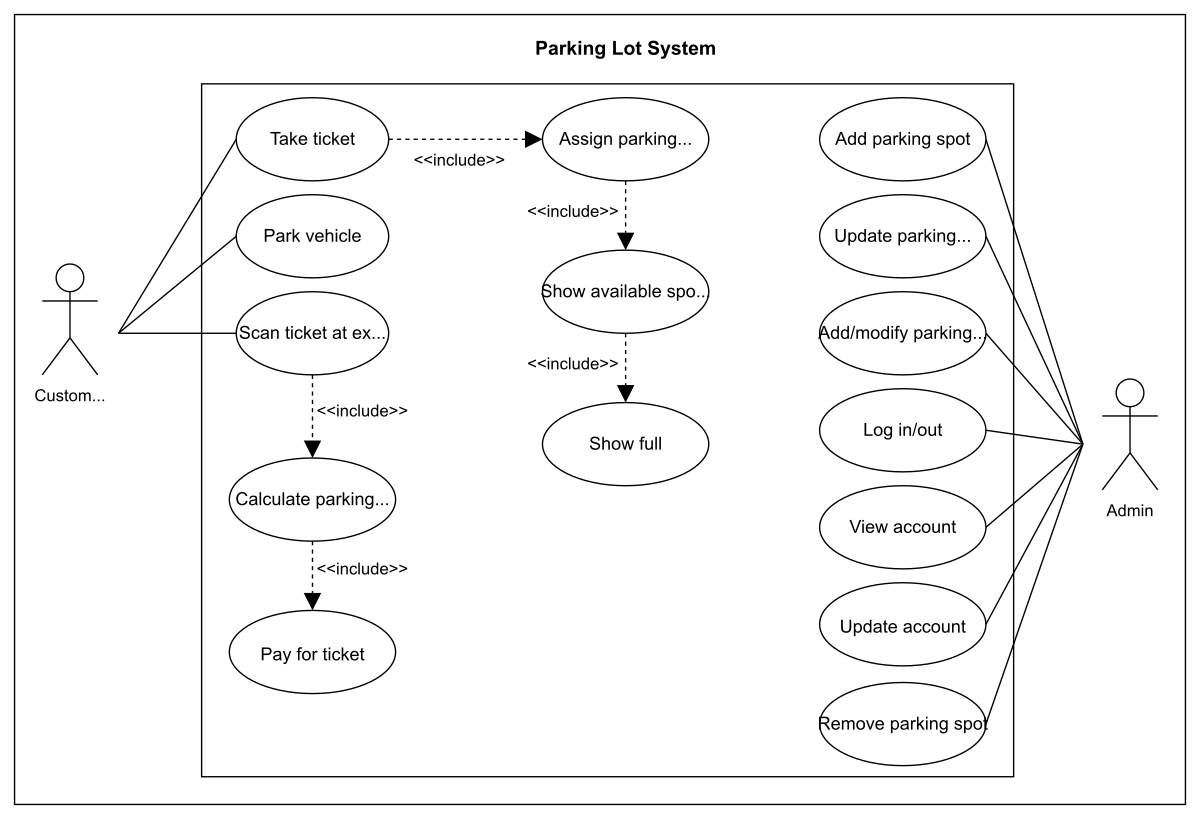
\includegraphics[width=0.5\textwidth]{Images/chapter_7/section_5098525681778688/5046737491066880.png}
 \caption{The use case diagram of the parking lot system}
\end{figure}

In the next lesson, we will discuss the class diagram with a detailed explanation of all classes and their relationship with each other.

% End of section content